\chapter{Literature Review}
This section of the report expands upon the theory behind the design of the system. Digital image processing and computer vision are a broad fields and so only concepts relevant to this system are detailed.

\section{Digital Images}
Unlike its analog predecessor the digital image consists of a discrete number of discrete valued data points called pixels. An image's resolution is defined how many pixels are in it and a pixel's value determines its colour. A pixel's value is also called its \emph{intensity} and lies within a spectrum of values, for example an 8-bit image can have pixel values $[0, 255]$. 

Digital images are often represented as a 2D array of values where each cell corresponds to an intesnity. In software this is how digital images are stored and manipulated. The image's array is $M\;pixels\times N\; pixels$ in size. Notice that in Figure \ref{fig:2Darray}, the lowest value is 0 (black) and the highest value is 255 (white). All other color that can be represented by 8-bits are between these two values.

\begin{figure}[ht!]
    \centering
    \begin{subfigure}[b]{0.5\linewidth}
      \centering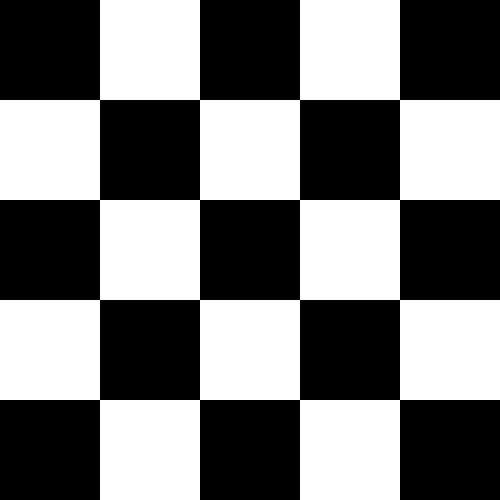
\includegraphics[width=150pt]{chessboard}
      \caption{\label{fig:fig1}}
    \end{subfigure}%
    \begin{subfigure}[b]{0.5\linewidth}
      \centering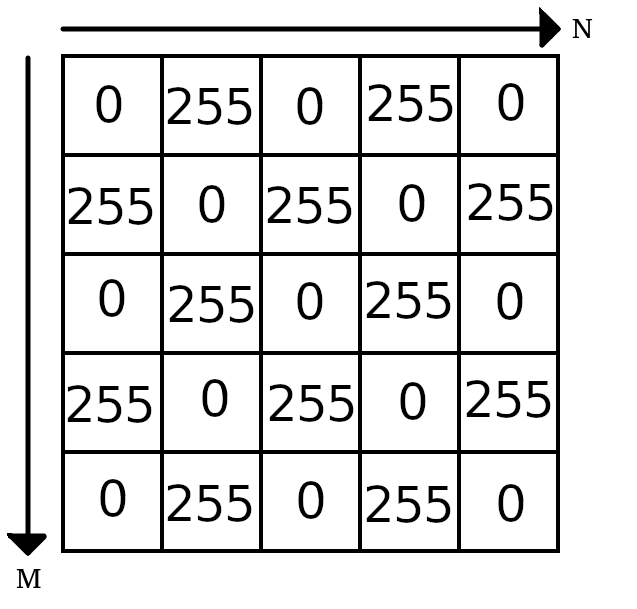
\includegraphics[width=150pt]{array2}
      \caption{\label{fig:fig2}}
    \end{subfigure}
    \caption{(\subref{fig:fig1}) A Simple 8-bit Image ~(\subref{fig:fig2}) Array Representation of Image.}
    \label{fig:2Darray}

\end{figure}
  

The 2D array representation allows pixels to be referenced by their relative position in the $M$ and $N$ directions. Furthermore, $M$ and $N$ may be substituted for something more familiar like the x and y-axis of a Cartesian plane. In fact, a digital image is just a two dimensional function (Equation \ref{eq:2Dfunc}), where each pixel is described by a coordinate (x,y) and an intensity (z) at that point.

\begin{equation}
    z = f(x,y)
    \label{eq:2Dfunc}
\end{equation}

This means that two dimnesional operations may be applied to a digital images. As a consequence images may be modelled as 3D surfaces. This is useful when trying to visualize rates of change in an image.

\begin{figure}[ht!]
  \centering
  \centering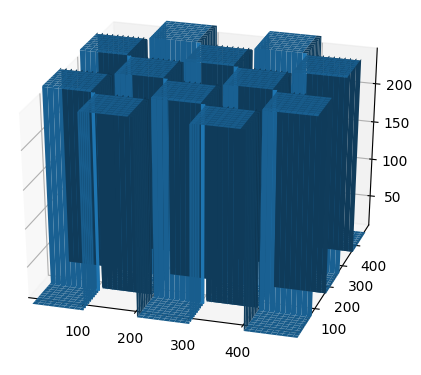
\includegraphics[width=150pt]{3Dchess}
  \caption{\label{fig:fig1} Surface Plot of Figure \ref{fig:fig1}\ref{sub@fig:fig1}}
\end{figure}




\section{Linear Filtering}

Filtering an image is a way to augment or extract information from it. Linear filters are a subset of operations that operate on a neighbourhood of pixels in an image. A filter's size determines the size of the neighbourhood to take as input for the operation.

Linear operations are characterized by two properties,

\begin{enumerate}
  \item They are shift invariant, meaning it doesn't matter where you apply the filter to an image, its effect is consistent.
  \item They preserve vector space operations, meaning it doesn't matter if they're applied before or after another linear operation, the result is the same.
\end{enumerate}

All linear filters operate on the same prinicpal, that is, they output a weighted average of their input. It is the weightings of a filter, known as \emph{filter coefficients}, that determine the effect of the filter. These weights are stored in a matrix called a \emph{mask} or \emph{kernel} that's then passed over the image. The mask is nearly always square so as to have a center which sits atop a reference pixel. The position of the reference pixel in the filtered image (output) will hold the result of the filter application that had that position at its center.

[SHOW FILTER OVER IMAGE, NEIGHBORHOOD, CENTER PIXEL, MASK ]
\begin{figure}[!ht]
  \begin{mdframed}
  \centering
  \centering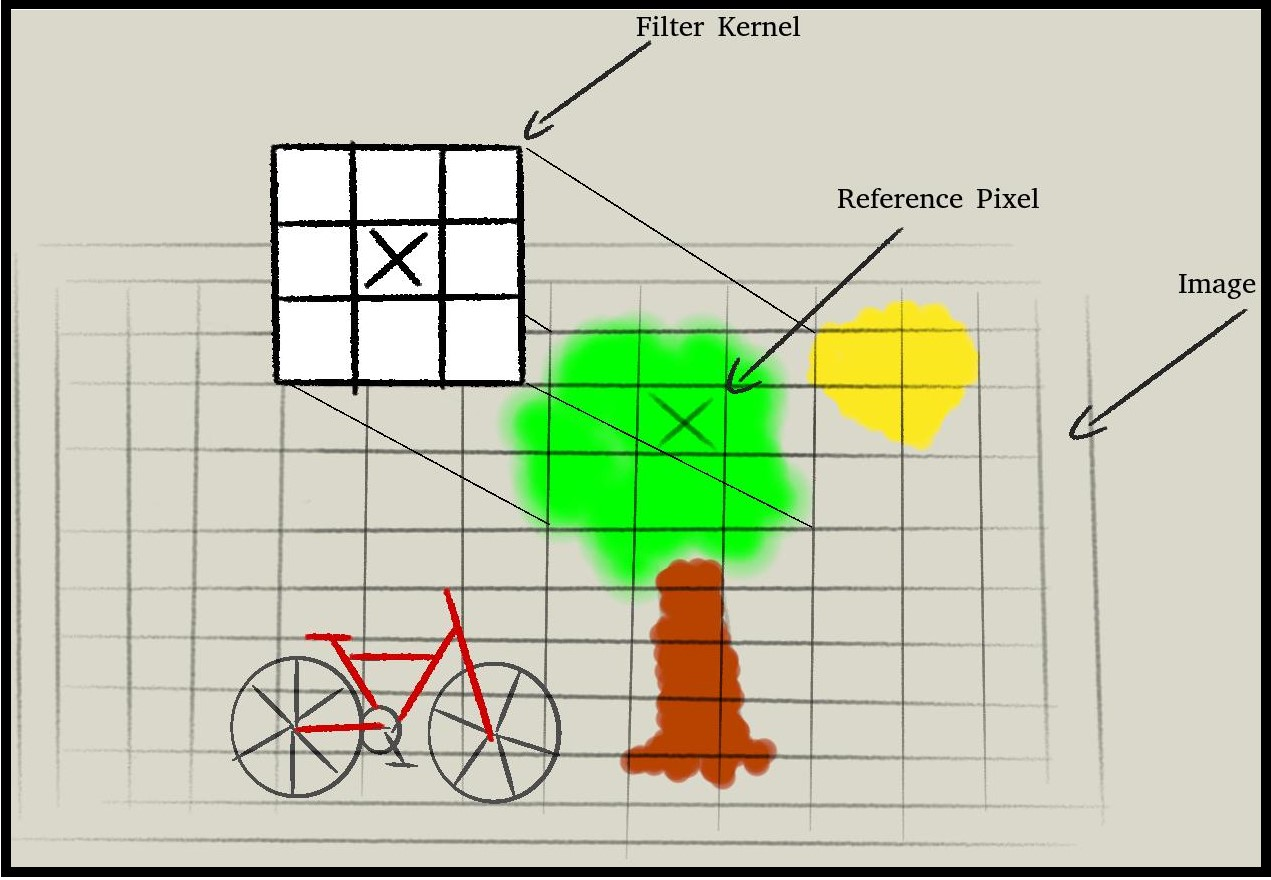
\includegraphics[width=350pt]{kernel_graphics}
  \end{mdframed}
  \caption{Application of a Filter Kernel to an Image}

\end{figure}

For example, a box filter simply outputs the average of its inputs by having all filter coefficients equal and then scaling the result by the sum of all weights. This is useful for smoothing images.

[ SHOW BOX FILTER MASK MATRIX ]
\begin{figure}
  \begin{gather}
    Kernel  = \frac{1}{\sum\limits_{i=0}^{M}\sum\limits_{j=0}^{N}c_{i,j}}
    \begin{bmatrix}
      c_{0,0} & c_{0,1} & \dots & c_{0,n} \\
      c_{1,0} & c_{1,1} & \dots & c_{1,n} \\
      \vdots & \vdots & \ddots & \vdots \\
      c_{m,0} & c_{m,1} & \dots & c_{m,n}
    \end{bmatrix}
  \end{gather}
  \caption{General Form of a Linear Filter}
\end{figure}


Here, the weights are evenly distributed and equal to the chosen weight divided by the sum of all weights. By passing this filter over an entire image the sharpness of the image is reduced as all the values are averages of their neighbourhood, giving a smoothing or blurring effect.

[ SHOW OUTCOME OF APPLYING BOX FILTER TO IMAGE  ]

\begin{figure}[ht!]
  \centering
  \begin{subfigure}[b]{0.5\linewidth}
    \centering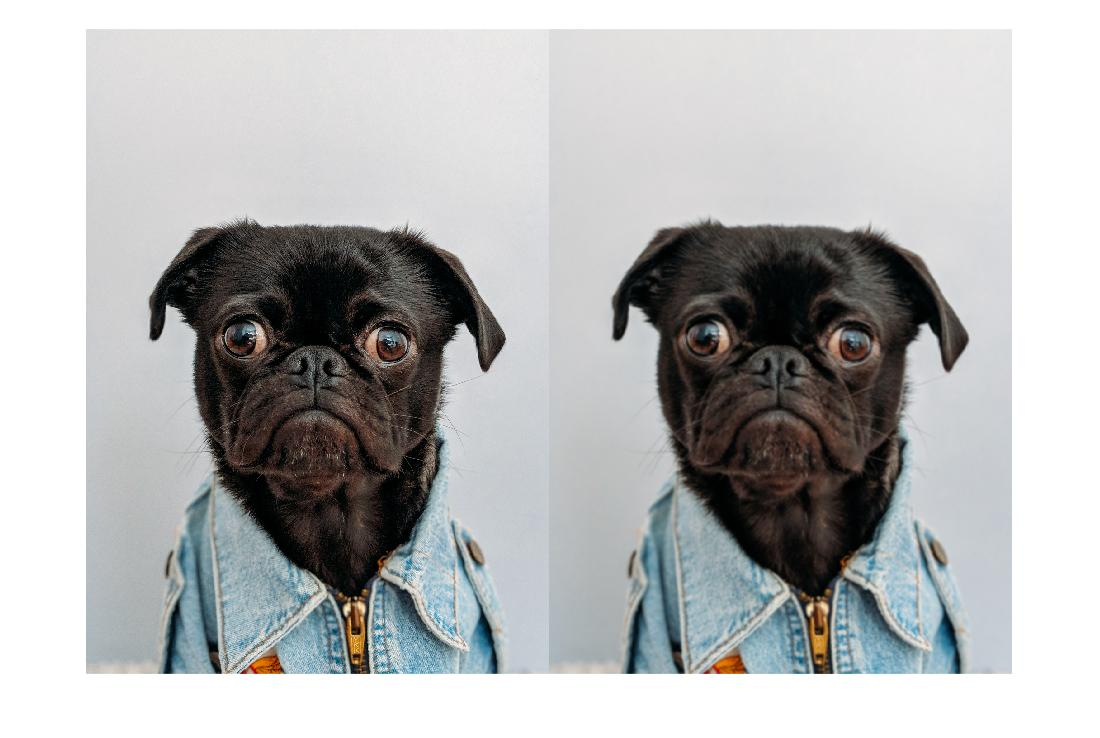
\includegraphics[width=150pt]{dogPug}
    \caption{Photo by Charles Deluvio on Unsplash}
    \label{fig:roughDog}
  \end{subfigure}
  \begin{subfigure}[b]{0.5\linewidth}
    \centering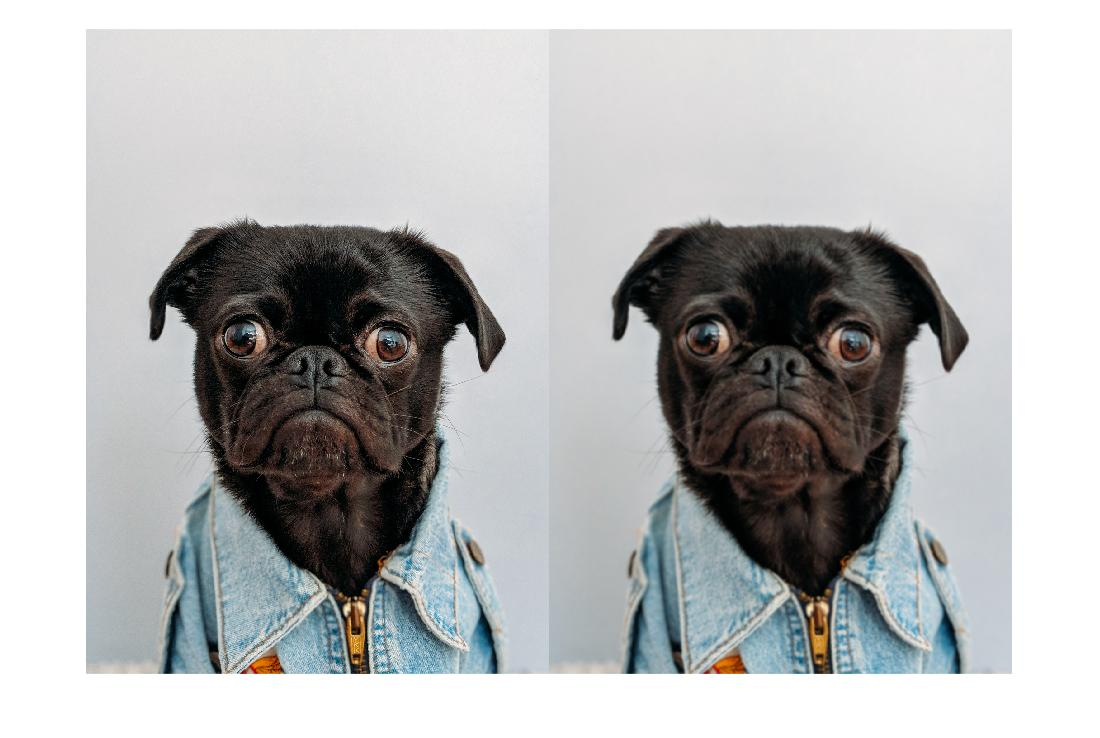
\includegraphics[width=150pt]{dogPug}
    \caption{Photo by Charles Deluvio on Unsplash}
    \label{fig:smoothDog}
  \end{subfigure}
  \caption{Application of Box Filter to RGB Dog}
  \label{fig:dogPug}
\end{figure}

The application of a linear filter $h(u,v)$ to an entire image $f(i,j)$, where $h(0,0)$ is the center of the filter mask and $f(0,0)$ is the target pixel beneath the masks center, may be described as follows

\begin{equation} \label{eq:1}
g(i,j) = \sum_{u=-k}^{k}\sum_{v = -l}^{l}f(i+u,j+v)h(u,v)
\end{equation}


where the dimensions of the filter kernel are $2k+1 \times 2l+1$. Filter kernels are nearly always odd dimensioned so as to have a center. This is because an asymmetric kernel (even numbered dimensions) will result in information being distorted because the output from the filter will be weighted unevenly by being placed in a reference pixel more one to one side than another.

[ SHOW RESULT OF USING ASYMMETRICAL KERNEL ] 



\subsection{Correlation}

Linear filtering may be notated more concisely by the \emph{correlation} operator.

\[g = f \otimes h\]

This operation measures the similarity between two signals (functions). We can think of both digital images and linear filters as signals. Performing correlation between them will yield an image where the highest values (pixel intensities) correspond to where the image and filter were most similar\cite{optimalKernel}.


[ SHOW EXAMPLE WITH SHARPENING FILTER ]

This operation is \emph{shift invariant}, which means that it does the same thing no matter where in an image it is applied. Therefore, correlation operations obey both the superposition principle

\[a(f_1 + f_2) = af_1 + af_2\]

and the shift invariance principle

\[g(i,j)=f(i+k,j+l) \Leftrightarrow\ (h\circ g)(i,j)=(h\circ f)(i+k,j+l)\]

This operation has the side effect of flipping both horizontally and vertically the location of output points relative to location the center point (\emph{reference point}) in the original image which may be undesirable.

[ SHOW EXAMPLE OF HOW CORRELATION FLIPS INPUT FOR OUTPUT ]

\subsection{Convolution}

Convolution is also a linear operation that is shift invariant. It is very similar to correlation except that the output signal from a convolution operation is not flipped relative to the input signal. It is described mathematically by the expression,

\[ g(i,j) = \sum_{u=-k}^{k}\sum_{v = -l}^{k}f(u,v)h(i-u,j-v)\]

We see that this is similar to equation \ref{eq:1} but that the filter $h(i,j)$ is the entity being shifted, furthermore it is flipped (note the negative signs), this results in the output's orientation being correct. Convolution may be notated with the following operator

\[g = f \ast h\]

[ SHOW EXAMPLE OF CONVOLUTION NOT FLIPPING OUTPUT ]


\section{Clustering}
This is a method of separating an image in disjoint sets (clusters). This is useful as we can semantically label different sections of an image according to their similarity.

[ SHOW EXAMPLE OF IMAGE SEGMENTED BY CLUSTERING ]

An entity’s  (for example a pixel) membership to a cluster is justified by it meeting some criteria that along with the rest of the cluster’s members. A simple example of this is a luster defined by its location in an image, all pixels in that region would belong to that cluster. This is a very simple criteria and often more sophisticated prerequisites must be met in order to classify a pixel's cluster. Entities like pixels or a neighbourhood of pixels' characteristics are represented in something called a feature vector.


\subsection{K-Means}
There are many methods by which to segment an image with clustering but K-Means is very popular for its simplicity and speed. K-means produces K clusters implemented as follows

    \begin{enumerate}
    \itemsep0em
        \item Place K points on the image randomly or with some educated guess. These points are the initial centroids for the K clusters.  
        \item Assign all data points to their nearest centroid.
        \item Update the centroids' positions as the mean of all data points in that class.
        \item Repeat steps 2 and 3 until cluster centroids no longer move (converge). 
    \end{enumerate}

K-means is guided by trying to limit the variance within each class. Variance is described by the expression

\begin{equation}\label{eq:2}
   V = \sum_{i=1}^k\sum_{x_j\in c_i}(x_j-\mu_i)^2 
\end{equation}

Where {$x_j$} are the data vectors, $c_i$ are the classes that the data point belong to and $\mu_i$ are the class centroids.

Because the K-Means algorithm is fast and the success of the segmentation depends on the initial placement of centroids, often the algorithm is performed many times with different initial conditions and the instance that yields the best results is used. 


[ SHOW EXAMPLE OF K-MEANS CLUSTERING BEING USED ]
\section{Gaussian Mixture Model}


\section{Morphology}

\section{Contours}

\section{Centroid Tracking}


